\documentclass[UTF8, 12pt]{ctexart}
% UTF8编码,ctexart现实中文
\usepackage{xcolor}
% 使用颜色
\definecolor{orange}{RGB}{255,127,0} 
\definecolor{violet}{RGB}{192,0,255} 
\definecolor{aqua}{RGB}{0,255,255} 
\usepackage{geometry}
\setcounter{tocdepth}{4}
\setcounter{secnumdepth}{4}
% 设置四级目录与标题
\geometry{papersize={21cm,29.7cm}}
% 默认大小为A4
\geometry{left=3.18cm,right=3.18cm,top=2.54cm,bottom=2.54cm}
% 默认页边距为1英尺与1.25英尺
\usepackage{indentfirst}
\setlength{\parindent}{2.45em}
% 首行缩进2个中文字符
\usepackage{setspace}
\renewcommand{\baselinestretch}{1.5}
% 1.5倍行距
\usepackage{amssymb}
% 因为所以
\usepackage{amsmath}
% 数学公式
\usepackage[colorlinks,linkcolor=black,urlcolor=blue]{hyperref}
% 超链接
\usepackage{pifont}
% 圆圈序号
\usepackage{tikz}
% 绘图
\author{Didnelpsun}
\title{多元函数微分学}
\date{}
\begin{document}
\maketitle
\pagestyle{empty}
\thispagestyle{empty}
\tableofcontents
\thispagestyle{empty}
\newpage
\pagestyle{plain}
\setcounter{page}{1}
\section{基本概念}
\subsection{平面与点}
\subsubsection{平面点集}

\textcolor{violet}{\textbf{定义:}}在平面上建立直角坐标系$xOy$,则平面上的点可用两个实数组的有序数组$(x,y)$表示,而二元函数$f(x,y)$的定义域是$(x,y)$为元素的几何,所以$f(x,y)$的定义域就是\textbf{平面上的点集}。

\subsubsection{距离}

\textcolor{aqua}{\textbf{定理:}}平面上任意两点$M_1(x_1,y_1)$与$M_2(x_2,y_2)$之间距离定义为$\rho(M_1,M_2)$\\$=\sqrt{(x_2-x_1)^2+(y_2-y_1)^2}$。

$\rho(M_1,M_2)$满足:

\begin{itemize}
    \item 非负性:$\rho(M_1,M_2)\geqslant0$。
    \item 对称性:$\rho(M_1,M_2)=\rho(M_2,M_1)$。
    \item 三角不等式:$\rho(M_1,M_3)\leqslant\rho(M_1,M_2)+\rho(M_2,M_3)$。
\end{itemize}

\subsubsection{邻域}

设$M_0$为平面上一点,$\delta>0$,则平面上以$M_0$为圆心,$\delta$为半径的圆的内部称为$M_0$的\textbf{$\delta$领域},记为$U(M_0,\delta)$。

若领域中去掉圆心$M_0$,称为$M_0$的\textbf{$\delta$去心邻域},记为$\mathring{U}(M_0,\delta)$。

\subsubsection{点的分类}

\textcolor{violet}{\textbf{定义:}}设$M$为平面上一个点,若存在$\delta>0$,使得$U(M,\delta)\subset E$,则$M$为点集$E$的\textbf{内点}。

\textcolor{violet}{\textbf{定义:}}若存在$\delta>0$,使得$U(M,\delta)\cap E=\varnothing$,则$M$为点集$E$的的\textbf{外点}。

\textcolor{violet}{\textbf{定义:}}若对任意$\delta>0$,$U(M,\delta)$即有$E$内的点也有外的点,则$M$为点集$E$的\textbf{边界点}。

\textcolor{violet}{\textbf{定义:}}$E$所有边界点的集合称为$E$的\textbf{边界},记为$\partial E$。对于任意一个点集$E$与其余集$E^C$有公共边界,即$\partial E=\partial E^C$。

\subsubsection{集合}

\textcolor{violet}{\textbf{定义:}}设$E$为一个平面点集,若存在常数$\delta>0$,使得$E\subset U(O,\delta)$,则$E$为\textbf{有界集},否则为\textbf{无界集}。

\textcolor{violet}{\textbf{定义:}}若$E$中的每个点都是$E$的内点,则$E$为\textbf{开集},若$E$的边界点都是$E$的点,则$E$为\textbf{闭集}。若一个点集是开集,则其余集为闭集,若一个点集为闭集,则其余集为开集。

\textcolor{violet}{\textbf{定义:}}若$E$中任意两点,都可用一条完全属于$E$的曲线将其两点连接,则$E$为\textbf{(道路)连通集},连通的开集为\textbf{开区域},一个开区域和其边界点的并集为\textbf{闭区域},统称\textbf{区域}。

\textcolor{violet}{\textbf{定义:}}若$E$内任意一条\textbf{简单闭曲线}的内部还在$E$内,则$E$为\textbf{单连通区域},否则为\textbf{多连通区域}。

\subsubsection{聚点}

\textcolor{violet}{\textbf{定义:}}对一个平面点集$E$,$M_0$为平面上一点,若对任意$\delta>0$,总有$\mathring{U}(M_0,\delta)\cap E\neq\varnothing$,即$M_0$的任意邻域中都含有异于$M_0$的$E$中的点,则$M_0$为$E$的\textbf{聚点}。

\textcolor{aqua}{\textbf{定理:}}非空开集的内点余边界点都是这个点集的聚点,闭区域的任意一点都是其聚点。

\textcolor{violet}{\textbf{定义:}}若存在$\delta>0$,使得$U(M_0,\delta)\cap E=\{M_0\}$,即如果$M_0$的某一邻域与点集$E$的交集是一个孤立的点$M_0$,则称$M_0$为$E$的\textbf{孤立点}。边界点要么是聚点要么是孤立点。

\subsection{极限}

对于一元函数的极限可用列举法,从两端逼近该点取极限,但是对于多元函数所处的邻域,逼近方向为无穷,所以不可能再通过取两个方向逼近的方式求极限。

从点集来看\textcolor{violet}{\textbf{定义:}}设二元函数$f(P)=f(x,y)$的定义域为$D$,$P_0(x_0,y_0)$为$D$聚点。若存在常数$A$,对于任意给定正数$\epsilon$,总存在正数$\delta$,使得当$P(x,y)\in D\cap\mathring{U}(P_0,\delta)$时,都有$\vert f(x,y)-A\vert<\epsilon$成立,则常数$A$为$f(x,y)$当$(x,y)\rightarrow(x_0,y_0)$时的极限,记为$\lim\limits_{(x,y)\to(x_0,y_0)}f(x,y)=A$或$f(x,y)\to A((x,y)\to(x_0,y_0))$。

如$\because xy\neq0$排除$xy$轴:$\lim\limits_{(x,y)\to(0,0)}\dfrac{\sqrt{xy+1}-1}{xy}=\lim\limits_{(x,y)\to(0,0)}\dfrac{xy+1-1}{xy(\sqrt{xy+1}+1)}$\\$=\lim\limits_{(x,y)\to(0,0)}\dfrac{1}{\sqrt{xy+1}+1}=\dfrac{1}{2}$。\medskip

从邻域来看\textcolor{violet}{\textbf{定义:}}若二元函数$f(x,y)$在$(x_0,y_0)$的去心邻域内有定义,且$(x,y)$以任意方式趋向$(x_0,y_0)$时,$f(x,y)$均趋向于$A$,则$\lim\limits_{\substack{x\to x_0\\y\to y_0}}f(x,y)=A$。

根据邻域的定义,由于函数$\lim\limits_{(x,y)\to(0,0)}\dfrac{\sqrt{xy+1}-1}{xy}$在坐标轴上无定义,则极限不存在。

此时两种定义就会有两种结论,所以为了避免这种定义不同的矛盾,就只会出现哪种定义下极限存在或都不存在的函数,如$\lim\limits_{\substack{x\to0\\y\to0}}(x^2+y^2)\sin\dfrac{1}{x^2+y^2}=0$。

从现实角度来看,点集定义是更合理的,若要求一根弯曲铁丝在某点的导数,第二种定义无法求,所以不合理。而第二种定义是从一元极限定义直接升级过来,所以有一定局限性。

\subsection{连续}

\textcolor{violet}{\textbf{定义:}}若$\lim\limits_{\substack{x\to x_0\\y\to y_0}}f(x,y)=f(x_0,y_0)$则称$f(x,y)$在点$(x_0,y_0)$处连续。

若不连续,则不讨论间断类型。

\subsection{偏导数}

当含有两个以及三个变量时,若求一个极限,则有多个变量同时趋向,所以多个变量同时在变。为了运算简单,就假定只有一个变量在变,其他变量固定,从而直接降低成一元变量,只对一个变量求导,从而就是偏导数。

\textcolor{violet}{\textbf{定义:}}设函数$z=f(x,y)$在点$(x_0,y_0)$的某邻域内有定义,若极限\\$\lim\limits_{\Delta x\to0}\dfrac{f(x_0+\Delta x,y_0)-f(x_0,y_0)}{\Delta x}$存在,则称此极限为函数$z=f(x,y)$在点$(x_0,y_0)$处对$x$的\textbf{偏导数},记为$\dfrac{\partial z}{\partial x}\bigg|_{\substack{x=x_0\\y=y_0}}$,$\dfrac{\partial f}{\partial x}\bigg|_{\substack{x=x_0\\y=y_0}}$,$z'\bigg|_{\substack{x=x_0\\y=y_0}}$或$f'_x(x_0,y_0)$。\medskip

$f'_x(x_0,y_0)=\lim\limits_{\Delta x\to0}\dfrac{f(x_0+\Delta x,y_0)-f(x_0,y_0)}{\Delta x}=\lim\limits_{x\to x_0}\dfrac{f(x,y_0)-f(x_0,y_0)}{x-x_0}$。

$f'_y(x_0,y_0)=\lim\limits_{\Delta y\to0}\dfrac{f(x_0,y_0+\Delta y)-f(x_0,y_0)}{\Delta y}=\lim\limits_{y\to y_0}\dfrac{f(x_0,y)-f(x_0,y_0)}{y-y_0}$。

\textcolor{violet}{\textbf{定义:}}若函数$z=f(x,y)$在区域$D$内的偏导数$f_x'(x,y)$、$f_y'(x,y)$仍具有偏导数,则其偏导数为函数$z=f(x,y)$的\textbf{二阶偏导数}。按照求导次序不同,有如下四个二阶偏导数。

$\dfrac{\partial}{\partial x}\left(\dfrac{\partial z}{\partial x}\right)=\dfrac{\partial^2z}{\partial x^2}=f''_{xx}(x,y)$,$\dfrac{\partial}{\partial y}\left(\dfrac{\partial z}{\partial y}\right)=\dfrac{\partial^2z}{\partial y^2}=f''_{yy}(x,y)$,

$\dfrac{\partial}{\partial y}\left(\dfrac{\partial z}{\partial x}\right)=\dfrac{\partial^2z}{\partial x\partial y}=f''_{xy}(x,y)$,$\dfrac{\partial}{\partial x}\left(\dfrac{\partial z}{\partial y}\right)=\dfrac{\partial^2z}{\partial y\partial x}=f''_{yx}(x,y)$。

其中$f''_{xy}(x,y)$和$f''_{yx}(x,y)$为\textbf{混合偏导数}。二阶以及以上的偏导数均为\textbf{高阶偏导数}。

\subsection{全微分}

\textcolor{violet}{\textbf{定义:}}若函数$z=f(x,y)$在点$(x,y)$的全增量$\Delta z=f(x+\Delta x,y+\Delta y)-f(x,y)$可表示为$\Delta z=A\Delta x+B\Delta y+o(\rho)$,其中$\rho=\sqrt{(\Delta x)^2+(\Delta y)^2}$,$AB$不依赖$\Delta x$,$\Delta y$而仅与$x,y$相关,则称函数$z=f(x,y)$在点$(x,y)$可微,而称$A\Delta x+B\Delta y$为函数$z=f(x,y)$在点$(x,y)$的\textbf{全微分},记为$\textrm{d}z$。

$\textrm{d}z=A\Delta x+B\Delta y=\dfrac{\partial z}{\partial x}\Delta x+\dfrac{\partial z}{\partial y}\Delta y=\dfrac{\partial z}{\partial x}\textrm{d}x+\dfrac{\partial z}{\partial y}\textrm{d}y$。

判断可微的步骤:

\begin{enumerate}
    \item 写出全增量$\Delta z=f(x_0+\Delta x,y_0+\Delta y)-f(x_0,y_0)$。
    \item 写出线性增量$A\Delta x+B\Delta y$,$A=f_x'(x_0,y_0)$,$B=f_y'(x_0,y_0)$。
    \item 写出极限$\lim\limits_{\substack{\Delta x\to0\\\Delta y\to0}}\dfrac{\Delta z-(A\Delta x+B\Delta y)}{\sqrt{(\Delta x)^2+(\Delta y)^2}}$,若极限等于0,则$z=f(x,y)$在点$(x_0,y_0)$可微,否则不可微。
\end{enumerate}

\subsection{偏导数连续性}

对$z=f(x,y)$,讨论其在某特殊点$(x_0,y_0)$处偏导数是否连续的步骤:

\begin{enumerate}
    \item 用定义法求$f_x'(x_0,y_0)$,$f_y'(x_0,y_0)$。(求某点偏导数)
    \item 用公式法求$f_x'(x,y)$,$f_y'(x,y)$。(求偏导函数)
    \item 计算$\lim\limits_{\substack{x\to x_0\\y\to y_0}}f_x'(x,y)$,$\lim\limits_{\substack{x\to x_0\\y\to y_0}}f_y'(x,y)$。(偏导函数求极限)
    \item 若$\lim\limits_{\substack{x\to x_0\\y\to y_0}}f_x'(x,y)=f_x'(x_0,y_0)$,$\lim\limits_{\substack{x\to x_0\\y\to y_0}}f_y'(x,y)=f_y'(x_0,y_0)$若成立则连续,否则不连续。
\end{enumerate}

\textbf{例题:}设$z=f(x,y)=\left\{\begin{array}{ll}
    (x^2+y^2)\sin\dfrac{1}{\sqrt{x^2+y^2}}, & x^2+y^2\neq0 \\
    0, & x^2+y^2=0
\end{array}\right.$,则四个结论中正确的个数为()。

\ding{172}$f(x,y)$在$(0,0)$处连续。\qquad\ding{173}$f'_x(0,0)$,$f'_y(0,0)$存在。

\ding{174}$f_x'(x,y)$,$f_y'(x,y)$在$(0,0)$处连续。\qquad\ding{174}$f(x,y)$在$(0,0)$可微。

$A.1$\qquad$B.2$\qquad$C.3$\qquad$D.4$

解:$\lim\limits_{\substack{x\to0\\y\to0}}(x^2+y^2)\sin\dfrac{1}{\sqrt{x^2+y^2}}=0=f(0,0)$。所以$A$正确。

$f_x'(0,0)=\lim\limits_{\Delta x\to0}\dfrac{f(0+\Delta x,0)-f(0,0)}{\Delta x}=\lim\limits_{\Delta x\to0}\dfrac{(\Delta x)^2\sin\dfrac{1}{\sqrt{(\Delta x)^2}}-0}{\Delta x}=$\\$\lim\limits_{\Delta x\to0}(\Delta x)\sin\dfrac{1}{\vert\Delta x\vert}=0$。同理$f'_y(0,0)=0$。

判断连续性,首先计算偏导数值,之前计算过:$f_x'(0,0)=f_y'(0,0)=0$;然后求偏导函数$f_x'(x,y)=2x\sin\dfrac{1}{\sqrt{x^2+y^2}}+(x^2+y^2)\cos\dfrac{1}{\sqrt{x^2+y^2}}\left(-\dfrac{1}{2}\right)\dfrac{2x}{\sqrt{(x^2+y^2)^3}}$\\$=2x\sin\dfrac{1}{\sqrt{x^2+y^2}}-\dfrac{x}{\sqrt{x^2+y^2}}\cos\dfrac{1}{\sqrt{x^2+y^2}}$,同理得$f_y'(x,y)=2y\sin\dfrac{1}{\sqrt{x^2+y^2}}$\\$-\dfrac{y}{\sqrt{x^2+y^2}}\cos\dfrac{1}{\sqrt{x^2+y^2}}$;最后一步查看偏导函数值与偏导数值是否相等,$\because\lim\limits_{\substack{x\to0\\y\to0}}2x\sin\dfrac{1}{\sqrt{x^2+y^2}}=0$,且$\lim\limits_{\substack{x\to0\\y\to0}}\dfrac{x}{\sqrt{x^2+y^2}}\cos\dfrac{1}{\sqrt{x^2+y^2}}$震荡,所以总的来说极限值不存在,就不会等于偏导数值,同理可得函数的偏导数在该点不连续。

要求一个函数在某点可微,首先$\Delta z=f(0+\Delta x,0+\Delta y)-f(0,0)=[(\Delta x)^2+(\Delta y)^2]\sin\dfrac{1}{\sqrt{(\Delta x)^2+(\Delta y)^2}}$。然后$A\Delta x+B\Delta y=f_x'(0,0)\Delta x+f_y'(0,0)\Delta y=0$。最后求极限$\lim\limits_{\substack{\Delta x\to0\\\Delta y\to0}}\dfrac{\Delta z-(A\Delta x+B\Delta y)}{\sqrt{(\Delta x)^2+(\Delta y)^2}}=\lim\limits_{\substack{\Delta x\to0\\\Delta y\to0}}\sqrt{(\Delta x)^2+(\Delta y)^2}\sin\dfrac{1}{\sqrt{(\Delta x)^2+(\Delta y)^2}}$\\$=0$,所以在此点可微。

综上正确的结论有\ding{172}\ding{173}\ding{175}三个,所以选$C$。

\section{多元函数微分法则}

\subsection{链式求导法则}

主要对显函数的微分。

多元函数链式求导法则与一元函数的求导法则类似。都是从因变量从中间变量走到自变量。一条路径是一个加项,多少条从因变量到所有自变量的路就有多少个加项。每条路上由不同的路段组成,若有$n$层中间变量,则有$n+1$路段,路段之间项是乘积形式,若变量只与一个变量有一条路,则是导数$\textrm{d}$,若一个变量到多个变量有多条路,则是偏导数$\partial$。

\begin{minipage}{0.65\linewidth}
    因变量$z$到$x$一共有两条路,所以两个和项。每条路都有两端,所以和项中有两个乘项。$z$到$uv$两个中间变量,所以是两个偏导$\dfrac{\partial z}{\partial u}$和$\dfrac{\partial z}{\partial v}$。$uv$都只有一条路直接连通$x$,所以都是导数$\dfrac{\textrm{d}u}{\textrm{d}x}$和$\dfrac{\textrm{d}v}{\textrm{d}x}$。一条路的每个路段的项相乘:$\dfrac{\partial z}{\partial u}\dfrac{\textrm{d}u}{\textrm{d}x}$和$\dfrac{\partial z}{\partial v}\dfrac{\textrm{d}v}{\textrm{d}x}$。最后将每条路段相加:$\dfrac{\textrm{d}z}{\textrm{d}x}=\dfrac{\partial z}{\partial v}\dfrac{\textrm{d}v}{\textrm{d}x}$。
\end{minipage}
\hfill
\begin{minipage}{0.25\linewidth}
    \begin{tikzpicture}[scale=1]
        \filldraw[black] (-0.25,0) node{$z$};
        \draw[black](0,0) -- (1,1) node[right]{$u$};
        \draw[black](0,0) -- (1,-1) node[right]{$v$};
        \draw[black](1.5,1) -- (2.5,0) node[right]{$x$};
        \draw[black](1.5,-1) -- (2.5,0);
    \end{tikzpicture}
\end{minipage} \medskip

\begin{minipage}{0.25\linewidth}
    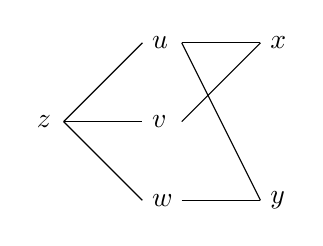
\begin{tikzpicture}[scale=1]
        \filldraw[black] (-0.25,0) node{$z$};
        \draw[black](0,0) -- (1,1) node[right]{$u$};
        \draw[black](0,0) -- (1,0) node[right]{$v$};
        \draw[black](0,0) -- (1,-1) node[right]{$w$};
        \draw[black](1.5,1) -- (2.5,1) node[right]{$x$};
        \draw[black](1.5,0) -- (2.5,1);
        \draw[black](1.5,-1) -- (2.5,-1) node[right]{$y$};
        \draw[black](1.5,1) -- (2.5,-1);
    \end{tikzpicture}
\end{minipage}
\hfill
\begin{minipage}{0.65\linewidth}
    因为因变量$z$到自变量$x,y$有较多条路径,所以分开分析。

    对于$x$,有$z-u-x$,所以这条路为$\dfrac{\partial z}{\partial u}\dfrac{\partial u}{\partial x}$,还有一条$z-v-x$,由于$v$只与$x$连通,所以是导数,该路为$\dfrac{\partial z}{\partial v}\dfrac{\textrm{d}v}{\textrm{d}x}$,所以$\dfrac{\partial z}{\partial x}=\dfrac{\partial z}{\partial u}\dfrac{\partial u}{\partial x}+\dfrac{\partial z}{\partial v}\dfrac{\textrm{d}v}{\textrm{d}x}$。、

    同理对于$y$,有$z-u-y$和$z-w-y$,且$u$有两条出路,$w$只有一条,所以$u$偏导,$v$导数,$\dfrac{\partial z}{\partial y}=\dfrac{\partial z}{\partial u}\dfrac{\partial u}{\partial y}+\dfrac{\partial z}{\partial w}\dfrac{\textrm{d}w}{\textrm{d}y}$。
\end{minipage} \medskip

无论$z$对谁求导也无论求了几阶到,求导过后的新函数仍具有与原函数完全相同的复合结构。

\textbf{例题:}设$z=f(e^x\sin y,x^2+y^2)$,其中$f$具有二阶连续偏导数,求$\dfrac{\partial^2z}{\partial x\partial y}$。

解:$\because\dfrac{\partial^2z}{\partial x\partial y}=\dfrac{\partial}{\partial y}\left(\dfrac{\partial z}{\partial x}\right)$,$\therefore\dfrac{\partial z}{\partial x}=f_1'\cdot e^x\sin y+f_2'\cdot2x$。

在求偏导时,将第一个中间变量记为$f_1$即之前的$u$,第二个中间变量记为$f_2$即之前的$v$。记$f$对$u$求偏导为$f_1'$,对$v$求偏导为$f_2'$同理二阶导也如此,下标为求导顺序。

$\dfrac{\partial^2z}{\partial x\partial y}=\dfrac{\partial(f_1'\cdot e^x\sin y)}{\partial y}+\dfrac{\partial(f_2'\cdot2x)}{\partial y}$。

其中$\dfrac{\partial(f_1'\cdot e^x\sin y)}{\partial y}=\dfrac{\partial f_1'}{\partial y}\cdot e^x\sin y+f_1'\cdot e^x\cos y$。所以难点就是$\dfrac{\partial f_1'}{\partial y}$。

求导路径$f_1'-1-y$和$f_1'-2-y$:$=(f_{11}''e^x\cos y+f_{12}''2y)\cdot e^x\sin y+f_1'\cdot e^x\cos y$。

其中$\dfrac{\partial(f_2'\cdot2x)}{\partial y}=2x\dfrac{\partial f_2'}{\partial y}$,求导路径$f_2'-1-y$和$f_2'-2-y$:$=2x(f_{21}''\cdot e^x\cos y+f_{22}''\cdot2y)$。

$\therefore\dfrac{\partial^2z}{\partial x\partial y}=(f_{11}''e^x\cos y+f_{12}''2y)\cdot e^x\sin y+f_1'\cdot e^x\cos y+2x(f_{21}''\cdot e^x\cos y+f_{22}''\cdot2y)$。

若$f$具有二阶连续偏导数,所以可以交换求导顺序,$f_{12}''=f_{21}''$。

化简:$=f_1'e^x\cos y+f_{11}''e^{2x}\sin y\cos y+2e^xf_{12}''(y\sin y+x\cos y)+4f_{22}''xy$。

\subsection{隐函数存在定理}

主要对隐函数的微分。隐函数的最大问题就是变量纠缠在一起,而公式法所得到的式子中变量都是独立的。

若对每个$x\in D$对应的函数值$y$总是唯一的,这样定义的函数为\textbf{单值函数}。若给定一个对应法则,按法则对$x$总有$y$与之对应,但是$y$不唯一,此时就不是函数,而确定一个\textbf{多值函数}。

只要满足着定义域的条件下,形如$y=f(x)$的函数就是\textbf{显函数},如$y=\sin x$。由方程$F(x,y)=0$确定的函数为\textbf{隐函数},如$x+y^3-1=0$显式表示为$y=\sqrt[3]{1-x}$。

\textcolor{violet}{\textbf{定义:}}设函数$F(x,y)$在点$P(x_0,y_0)$的某一邻域内具有连续偏导数,$F(x_0,y_0)$\\$=0$,$F_y'(x_0,y_0)\neq0$,则方程$F(x,y)=0$在点$(x_0,y_0)$的某一邻域内能唯一确定一个连续且具有连续导数的函数$y=f(x)$,满足$y_0=f(x_0)$。

\textcolor{violet}{\textbf{定义:}}二元隐函数求导公式:$\dfrac{\textrm{d}y}{\textrm{d}x}=-\dfrac{F_x'}{F_y'}$。

因为$y=y(x)$,所以对$F(x,y)$进行求导:$F_x'\cdot1+F_y'\cdot\dfrac{\textrm{d}y}{\textrm{d}x}=0$,就解出隐函数求导公式,$F_y'(x_0,y_0)\neq0$是定理关键。

如给出一个圆的方程$F(x,y)=x^2+y^2-1=0$,$F_x'=2x$,$F_y'=2y$,$F(0,1)=0$,$F'_y(0,1)=2\neq0$。所以在$(0,1)$和$(0,-1)$是单值的,从而能确定一个连续导数的隐函数,而在$(\pm1,0)$的邻域内不存在,因为其切线是竖直的。

\textcolor{violet}{\textbf{定义:}}设函数$F(x,y,z)$在点$P(x_0,y_0,z_0)$的某一邻域内具有连续偏导数,$F(x_0,y_0,z_0)=0$,$F_z'(x_0,y_0,z_0)\neq0$,则方程$F(x,y,z)=0$在点$(x_0,y_0,z_0)$的某一邻域内能唯一确定一个连续且具有连续导数的函数$z=f(x,y)$,满足$z_0=f(x_0,y_0)$。

\textcolor{violet}{\textbf{定义:}}三元隐函数求导公式:$\dfrac{\partial z}{\partial x}=-\dfrac{F_x'}{F_z'}$,$\dfrac{\partial z}{\partial y}=-\dfrac{F_y'}{F_z'}$。

因为$x$是$x$的函数,$y$是$y$的函数,$z$是$xy$的函数。所以$F_x'\cdot1+F_z'\cdot\dfrac{\partial z}{\partial x}=0$,解得$\dfrac{\partial z}{\partial x}=-\dfrac{F_x'}{F_z'}$。同理$F_y'\cdot1+F_z'\cdot\dfrac{\partial z}{\partial y}$也可得。

\textbf{例题:}设$z=f(x,y)$是由方程$z-y-x+xe^{z-y-x}=0$所确定的二元函数,求$\textrm{d}z$。

解:$\textrm{d}z=\dfrac{\partial z}{\partial x}\textrm{d}x+\dfrac{\partial z}{\partial y}\textrm{d}y$。其中$F_x'=-1+e^{z-y-x}-xe^{z-y-x}$,$F_y'=-1-xe^{z-y-z}$,$F_z'=1+xe^{z-y-x}$。

直接代入:$\dfrac{\partial z}{\partial x}\textrm{d}x+\dfrac{\partial z}{\partial y}\textrm{d}y=-\dfrac{F_x'}{F_z'}-\dfrac{F_y'}{F_z'}=\dfrac{1+(x-1)e^{z-y-x}}{1+xe^{z-y-x}}+1$。

\textbf{例题:}已知函数$z=f(x,y)$的全微分$\textrm{d}z=2x\,\textrm{d}x+\sin y\,\textrm{d}y$且$f(1,0)=2$,求$f(x,y)$。

解:$\because\textrm{d}z=2x\,\textrm{d}x+\sin y\,\textrm{d}y$,$\therefore\dfrac{\partial z}{\partial x}=2x$,$\dfrac{\partial z}{\partial y}=\sin y$。

对偏导进行积分:$f(x,y)=x^2+\varphi(y)$,$\dfrac{\partial(x^2+\varphi(y))}{\partial y}=\varphi'(y)=\sin y$。

又$\varphi(y)=-\cos y+C$,$f(x,y)=x^2-\cos y+C$,代入$f(1,0)=2$。

$C=2$,$f(x,y)=x^2-\cos y+2$。

\section{多元函数极值最值}

\subsection{概念}

\textcolor{violet}{\textbf{定义:}}若存在$(x_0,y_0)$的某个邻域,使得在该邻域内的任意一点$(x,y)$均有$f(x,y)\leqslant f(x_0,y_0)$或$f(x,y)\geqslant f(x_0,y_0)$成立,则称$(x_0,y_0)$为$f(x,y)$的\textbf{广义的极大值点/极小值点},$f(x_0,y_0)$为$f(x,y)$的\textbf{广义的极大值/极小值}。

\textcolor{violet}{\textbf{定义:}}若存在$(x_0,y_0)$的某个去心邻域,使得在该邻域内的任意一点$(x,y)$均有$f(x,y)<f(x_0,y_0)$或$f(x,y)>f(x_0,y_0)$成立,则称$(x_0,y_0)$为$f(x,y)$的\textbf{真正的极大值点/极小值点},$f(x_0,y_0)$为$f(x,y)$的\textbf{真正的极大值/极小值}。

\textcolor{violet}{\textbf{定义:}}设$(x_0,y_0)$为$f(x,y)$定义域内一点,若对于$f(x,y)$的定义域内任意一点$(x,y)$均有$f(x,y)\leqslant f(x_0,y_0)$或$f(x,y)\geqslant f(x_0,y_0)$成立,则称$(x_0,y_0)$为$f(x,y)$的\textbf{广义的最大值点/最小值点},$f(x_0,y_0)$为$f(x,y)$的\textbf{广义的最大值/最小值}。

\textcolor{violet}{\textbf{定义:}}设$(x_0,y_0)$为$f(x,y)$定义域内一点,若对于$f(x,y)$的定义域内任意一个异于$(x_0,y_0)$的点$(x,y)$均有$f(x,y)<f(x_0,y_0)$或$f(x,y)>f(x_0,y_0)$成立,则称$(x_0,y_0)$为$f(x,y)$的\textbf{真正的最大值点/最小值点},$f(x_0,y_0)$为$f(x,y)$的\textbf{真正的最大值/最小值}。

\subsection{无条件极值}

\textcolor{aqua}{\textbf{定理:}}二元函数取极值的必要条件:设$z=f(x,y)$在点$(x_0,y_0)$一阶偏导数存在且取极值,则$f_x'(x_0,y_0)=0$,$f_y'(x_0,y_0)=0$。三元及以上可以类推。

\textcolor{aqua}{\textbf{定理:}}二元函数取极值的充分条件:若对函数求二阶偏导$\left\{\begin{array}{l}
    f_{xx}''(x_0,y_0)=A \\
    f_{xy}''(x_0,y_0)=B \\
    f_{yy}''(x_0,y_0)=C
\end{array}\right.$,则$\Delta=B^2-AC=\left\{\begin{array}{l}
    <0\Rightarrow\text{极值}\left\{\begin{array}{l}
        A<0\Rightarrow\text{极大值} \\
        A>0\Rightarrow\text{极小值}
    \end{array}\right. \\
    >0\Rightarrow\text{非极值} \\
    =0\Rightarrow\text{方法失效,使用定义法}
\end{array}\right.$。只适用于二元函数极值。

\textbf{例题:}求函数$f(x,y)=x^4+y^4-(x+y)^2$的极值。

解:$f_x'=4x^3-2(x+y)=0$,$f_y'=4y^3-2(x+y)=0$,解得$x=y=-1,0,1$。

$f_{xx}''=12x^2-2$,$f_{xy}''=-2$,$f_{yy}''=12y^2-2$。各自代入:

$P_1:A_1=10,B_1=-2,C_1=10,\Delta=B_1^2-A_1C_1=-96<0,A_1>0$,极小。

同理$P3$也是极小值点。极小值为-2。

$P2:A_2=-2,B_2=-2,C_2=-2,\Delta_2=B_2^2-A_2C_2=0$。该方法失效。

取$y=x$的路径,$f(x,y)=f(x,x)=2x^4-4x^2=2x^2(x+\sqrt{2})(x-\sqrt{2})<0$。

取$y=-x$的路径,$f(x,y)=f(x,-x)=2x^4>0$。而$f(0,0)=0$。

所以不同的路径上有大于该值的也有小于该值的,所以该点不为极值点。

% \subsubsection{隐函数}

% \subsubsection{显函数}

\subsection{条件极值与拉格朗日乘数法}

求目标函数$u=f(x,y,z)$在一组条件函数$\varphi_1(x,y,z)=0,\varphi_2(x,y,z)=0,\cdots,\varphi_n(x,y,z)=0$下的最值,则:

\begin{enumerate}
    \item 构造辅助函数带$\lambda_i$:$F(x,y,z,\lambda_1,\lambda_2,\cdots,\lambda_n)=f(x,y,z)+\lambda_1\varphi_1(x,y,z)+$\\$\lambda_2\varphi_2(x,y,z)+\lambda_n\varphi_n(x,y,z)$,其中$\lambda_i\varphi_i$为\textbf{拉格朗日乘数}。
    \item 对函数依次对$x,y,z,\lambda_i$求偏导并令为0:$F_x'=f_x'+\lambda_1\varphi_{1x}'+\lambda_2\varphi_{2x}'+\cdots+\lambda_n\varphi_{nx}'=0$,$F_y'=f_y'+\lambda_1\varphi_{1y}'+\lambda_2\varphi_{2y}'+\cdots+\lambda_n\varphi_{ny}'=0$,$F_z'=f_z'+\lambda_1\varphi_{1z}'+\lambda_2\varphi_{2z}'+\cdots+\lambda_n\varphi_{nz}'=0$,$F_{\lambda_i}'=\varphi_i(x,y,z)=0$。一共$3+n$个方程。
    \item 解上述方程组得备选点$P_i$,$i=1,2,\cdots,n$,并求$f(P_i)$并取其最大值$m_{\max}$和最小值$u_{\min}$。
\end{enumerate}

\textbf{例题:}求函数$u=xyz$在约束条件$\dfrac{1}{x}+\dfrac{1}{y}+\dfrac{1}{z}=\dfrac{1}{a}$($x>0,y>0,z>0,a>0$)下的最小值。

解:令$F(x,y,z,\lambda)=xyz+\lambda\left(\dfrac{1}{x}+\dfrac{1}{y}+\dfrac{1}{z}-\dfrac{1}{a}\right)$。

令$F_x'=yz+-\dfrac{\lambda}{x^2}=0$,$F_y'=xz+-\dfrac{\lambda}{y^2}=0$,$F_z'=xy+-\dfrac{\lambda}{z^2}=0$,$F_\lambda'=\dfrac{1}{x}+\dfrac{1}{y}+\dfrac{1}{z}-\dfrac{1}{a}=0$。

解得$x=y=z=3a$,从而最小值为$u_{\min}=27a^3$。

% \subsubsection{闭区域边界最值}

% \subsubsection{闭区域上最值}

\end{document}
